% First draft: 1977_anhui_science_q9_fig1 (rectangle, division points).
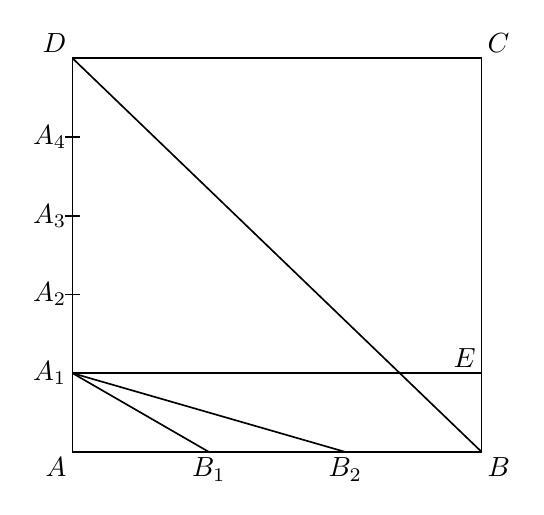
\begin{tikzpicture}[x=1cm,y=1cm,font=\normalsize,
 geometry edge/.style={solid,line width=.6pt},
 geometry mark/.style={solid,line width=.6pt},
 geometry label/.style={font=\normalsize,inner sep=2pt}]
\coordinate (A) at (0.0000,0.0000);
\coordinate (B) at (5.1962,0.0000);
\coordinate (C) at (5.1962,5.0000);
\coordinate (D) at (0.0000,5.0000);
\coordinate (A1) at (0.0000,1.0000);
\coordinate (A2) at (0.0000,2.0000);
\coordinate (A3) at (0.0000,3.0000);
\coordinate (A4) at (0.0000,4.0000);
\coordinate (B1) at (1.7321,0.0000);
\coordinate (B2) at (3.4641,0.0000);
\coordinate (E) at (5.1962,1.0000);
\draw[geometry edge] (A)--(B)--(C)--(D)--cycle;
\draw[geometry edge] (A1)--(E);
\draw[geometry edge] (A1)--(B1);
\draw[geometry edge] (A1)--(B2);
\draw[geometry edge] (D)--(B);
\draw[geometry mark] (-0.0900,2.0000)--(0.0900,2.0000);
\draw[geometry mark] (-0.0900,3.0000)--(0.0900,3.0000);
\draw[geometry mark] (-0.0900,4.0000)--(0.0900,4.0000);
\node[geometry label,below left] at (A) {$A$};
\node[geometry label,below right] at (B) {$B$};
\node[geometry label,above right] at (C) {$C$};
\node[geometry label,above left] at (D) {$D$};
\node[geometry label,left] at (A1) {$A_1$};
\node[geometry label,left] at (A2) {$A_2$};
\node[geometry label,left] at (A3) {$A_3$};
\node[geometry label,left] at (A4) {$A_4$};
\node[geometry label,below] at (B1) {$B_1$};
\node[geometry label,below] at (B2) {$B_2$};
\node[geometry label,above left] at (E) {$E$};
\end{tikzpicture}
